% 02/01 moved Lemma 3.3.2 to Section 3.7
% 02/01 changed according to ref No.2
% 02/05 changed from .emf to n.png
% 02/06 changed according to ref No.2 (by Makimoto)

%%%%%%%%%%%%%%%
%   Block    %%
%%%%%%%%%%%%%%%
\chapter{Optimal Slice of a Block Trade}\label{chap_b}

%%%%% local definition
\def\keymtx{\A^{-1}\S}

%%%%%%%%%%%%%%%%%%%%%%
%\newpage

%\vspace*{0.5cm}

%\begin{center}
%{\large {\bf Optimal Slice of a Block Trade}}
%\end{center}

%\vspace*{0.5cm}

\begin{quote}
{\bf Abstract} \quad In liquidation of a block trade, it is common to divide execution in order to minimize total transaction cost, balancing market impact costs and volatility effects.  This chapter formulates the execution scheduling as a static optimization problem assuming linear market impact and derives explicit solutions. We show that optimal execution duration and average cost are increasing functions of the initial portfolio size, which is consistent with trading practice and empirical studies.  Our model provides explicit solutions for minimum liquidity adjusted value at risk (L-VaR), which is particularly useful for risk management.

\vspace*{0.5cm}

\end{quote}

%%%%%%%%%%%%%%%%%
\section{Introduction}\label{sec_b1}

In various aspects of financial decision-making from risk management to trading, it is commonly assumed that any trade can be executed around a prevailing price within a short period of time.  However in practice, we sometimes face situations in which market cannot fully absorb all the trading needs of a large portfolio.  In such cases, asset liquidity risk, defined as the potential deviation between market price and executed price, becomes significant.  Liquidity risk has attracted much attention since the LTCM 1998 disaster, as described in Jorion (2000).  Conventional VaR measures should be extended to account for liquidity risk as well as optimal trading strategies.  This leads to the concept of L-VaR, a liquidity-adjusted risk measure. 

This chapter derives explicit solutions of optimal execution strategy under asset liquidity risk.  It extends the work of Almgren and Chriss (1999), who derive a measure of L-VaR.  Almgren and Chriss obtain optimal execution strategies by considering the trade-off between immediate liquidation, which entails no price risk but has high market impact, and slow liquidation, which minimizes market impact but exposes the portfolio to price risk.  Their approach, however, has the unrealistic property that the time scale of optimal trading is independent of the initial portfolio size.  Intuition suggests that larger portfolios should trade more slowly and that total execution costs should grow superlinearly with portfolio size.

In contrast, our model has several advantages.  First, we succeeded in making optimal execution duration an endogenous increasing function of whole trading size.  Second, our transaction cost grows superlinearly with whole trading size, consistent with intuition.  Third, our results are immediately applicable to existing risk management framework and provides explicit solution for minimum L-VaR.  Also, although this chapter uses an example of liquidation of a block of common stock, results can be extended over wider problems on liquidation of any large block of assets.

Since asset liquidity risk is a highly complicated problem, there used to be a large gap between practice and theory.  On the practice side, it is known that in liquidation of a block trade portfolio, traders generally divide the whole trade into small orders in order to reduce his cost.  In doing so, it is common to take a longer time for larger trades.  Also, BARRA (1997)'s analysis on quote driven market and Mannen and Uno (2000)'s analysis on order driven market show that the quoted premium of a block trade in the real market is an increasing function of whole trading size, and the marginal increment is a decreasing function (i.e., the first derivative is positive and the second derivative is negative).  

On the theory side,  Collins and Fabozzi (1991) proposed a conceptual framework, which decomposes trading cost into execution cost and opportunity cost.  According to their research, quick execution suffers huge execution cost, while slow execution creates large opportunity cost from price movement risk.  Therefore a trader chooses the best strategy that balances these two factors in determining execution schedule.

Subsequent studies investigated more detailed theory.  Bertsimas and Lo (1998) derived the optimal execution strategy of a large block of common stock over a fixed time horizon by dynamic programming.  However, they analyzed only risk neutral traders because of computational complexity of dynamic programming.  So, they just minimized the expectation value of execution cost, but did not consider price movement risk, and therefore, no reasonable guidance on the duration of execution was provided.  On the other hand, Grinold and Kahn (1999) and Almgren and Chriss (1999) took the sum of execution cost and opportunity cost of the whole trade, as the objective function to minimize, and derived a static optimal execution strategy.  Although they studied risk averse traders, optimal execution duration and average cost are still independent of whole trading size, which contradicts the result of BARRA (1997) and Mannen and Uno (2000).  Further, Grinold and Kahn (1999) contradicts their own statement that risk increases as square root of time, since their risk measured in variance, in fact, increases linearly.  This is crucial because the time dependency of cost and risk determines the optimal execution strategy.

 To the contrary, in order to bridge the gap between theory and practice, this chapter modifies objective function in a practical manner, which reflects the reality of the order driven market, and obtains a reasonable relationship between transaction cost and whole trading size.  Specifically, we extend the results on optimal execution strategy derived by Grinold and Kahn (1999) and Almgren and Chriss (1999).  As mentioned above, the explicit solutions obtained in the earlier work have the unrealistic properties that the time scale of optimal execution strategy is independent of whole trading size, and the total cost of trading is linear in whole trading size. 

There are two possible ways to capture these effects in a quantitative model. One way is to modify the cost functions to be nonlinear.  Another way is to change the weighting of cost uncertainty from a mean-variance model based on a smooth utility function, to a penalty based on standard deviation, which is more in the spirit of VaR models.  This approach was briefly discussed in Almgren and Chriss (1999) where it was observed that solutions could be obtained graphically on the efficient frontier, but explicit solutions were not obtained due to the nonlinearity of the problem, nor were the properties of these solutions explored.

For the standard deviation model, we obtain explicit solutions both for the single-asset case and for a multi-asset portfolio model in the form of pure exponentials.  The explicit form obtained for the coefficients shows that the characteristic time increases as whole trading size to the two-thirds power, and total cost increases as whole trading size to the four-thirds power, both consistent with intuition.

The biggest problem with this VaR-type weighting of risk is that the solutions  do not satisfy the ``principle of optimality": solutions computed statically at the start of trading are no longer optimal if reevaluated in the course of execution. Although formally this makes the solutions invalid, and calls for the use of a dynamic programming method, these solutions are useful in practice because of the following advantages:
\begin{itemize}
 \item Statically optimized execution can be used as a benchmark, i.e., actual trading strategy
might be changed as new information arrives and the performance of a strategy change can be
evaluated by comparing the cost to that of static optimal execution strategy.
 \item Statically optimized execution is sometimes a reasonable choice in program trading, i.e., it is
technically difficult to record all the history of price and profit and change the strategy
dynamically especially in a portfolio trade.  Therefore, static optimal execution strategy is a good
alternative in practical trading.
\end{itemize}

This chapter is organized as follows.  In the next section, we formulate the cost minimization problem.  Section \ref{sec_b3} is devoted to derive the optimal execution strategy for general case.  The case when we have limit to the volume executable instantaneously is studied in Section \ref{sec_b4}.  Section \ref{sec_b5} discusses the principle of optimality.  Finally in Section \ref{sec_b6}, we conclude the analysis.

%%%%%%%%%%%%%%%%%%%%%%%%
\section{Formulation of Optimization}\label{sec_b2}

 Let $(\Omega, \calF, Q)$ be a probability space with a filtration $\{ \calF_t \}$ which satisfies usual conditions.  Suppose we would like to liquidate a portfolio of $N$ assets and whole trading size of asset $i$ is $V_i\ (i=1,\cdots,N)$.  Let $P_i(t)\ (i=1,\cdots,N)$ denote $\{ \calF_t \}$-adapted stock's fair value process.  Similar to the standard option pricing theory, the stock price process is assumed to follow standard Brownian motion with volatility $\sigma_i$ and correlation $\rho_{ij}$.  Drift term is considered to be zero because the time frame is short.
 So, the stock's fair value processes are represented as
\begin{eqnarray*}
  & & dP_i(t) = \sigma_i dB_i(t), \quad i=1,\cdots,N, \\
  & & dB_i(t) dB_j(t) = \rho_{ij} dt, \quad i,j=1,\cdots,N.
\end{eqnarray*}
 Let $v_i(t)\ (i=1,\cdots,N)$ denote the selling volume of asset $i$ at time $t$.
 Because of the order quantity constraints,
\begin{equation}\label{eq_b1}
  \int_0^\infty v_i(t) dt = V_i, \qquad i=1,\cdots,N.
\end{equation}

 In the rest of the chapter, we consider total transaction cost as the sum of execution cost and opportunity cost, and study the static minimization of transaction cost under this framework.  More precisely, we look for $v_i(t)$ which minimizes transaction cost among all trading strategy that is pre-determined at $t=0$.

 Regarding execution cost, the main factor that can be controlled by order slicing is market impact, the difference between observed price at the market and the stock's fair value.  Holthausen et al.~(1987) and Uno and Yamada (1993) say that market price tends to overshoot with a block trade, and therefore, market impact should be divided into temporary and permanent components.  Further, several features are known regarding the market impact in an order driven market, such as the Japanese market.  First, according to Copeland and Galai (1983), a limit order can be considered as a free option contract, and so, only a part of demand and supply are placed as limit orders at one time.  Therefore, a trader has to wait until orders on the opposite side appear.  Actually, Biais et al.~(1995) observed that there are few limit orders at prices far from the market price.  Second, while a quote driven market allows a trader to negotiate prices with a market maker according to trading volume, an order driven market does not have a function to negotiate price and trading volume, which forces traders to repeat small execution.  Also, if anonymity is guaranteed in an order driven market, repeating execution is thought to leak less information than a bulk execution.  

In summary, the advantages of order slicing are 1) avoiding temporary
market impact, 2) waiting for all the potential orders to appear, and 3)
concealing one's trade.  Therefore, this chapter separates market impact
into temporary and permanent component, sets a limit to the volume
executable instantaneously, and assumes each component to be a linear
function of trading volume within moderate volume and time.  Choice
between market order and limit order is certainly another important
factor in optimal execution.  However, this chapter regards it as a
tactical decision after the order slice is fixed, and excludes it from
the scope of the research since it is common to place orders only around
a prevailing price as mentioned above.  Specifically, we introduce
coefficients below.

\vspace{3mm}

\begin{tabular}{l}
 $a_i>0\ (i=1,\cdots,N)$ : temporary impact coefficient of asset $i$, \\ [3mm]
 $b_i>0\ (i=1,\cdots,N)$ : permanent impact coefficient of asset $i$.
\end{tabular}

\vspace{3mm}

\noindent Since temporary impact depends only on the momentary trade and permanent impact depends on the accumulated volume traded up to that moment, total market impact at time $t$ can be represented as
\[
  \sum_{i=1}^N v_i(t) \left\{ a_i v_i(t) + b_i \int_0^t v_i(s) ds \right\}.
\]
 Therefore, market impact over the execution period becomes
\begin{eqnarray}
  \mbox{(market impact)}
  & = & \int_0^\infty \sum_{i=1}^N v_i(t) \left\{ a_i v_i(t) + b_i \int_0^t v_i(s) ds \right\} dt \nonumber \\
  & = & \int_0^\infty \v(t)^\top \A \v(t) dt +\frac{1}{2} \V^\top \B \V \label{eq_b16}
\end{eqnarray}
where $\v(t)=(v_1(t),\cdots,v_N(t))^\top$, $\V=(V_1,\cdots,V_N)^\top$,
$\A = \mbox{Diag}(a_1,\cdots,a_N)$, $\B= \mbox{Diag}(b_1,\cdots,b_N)$.
 Here, $\mbox{Diag}(z_1,\cdots,z_N)$ denotes an $N \times N$ diagonal matrix whose diagonal element is
$z_i\ (i=1,\cdots,N)$ and $\top$ denotes transpose.

 Meanwhile, regarding opportunity cost, price movement risk is often measured by a multiple of standard deviation as VaR, which has the same dimension as the price itself.  This risk measurement has the following advantages:
\begin{itemize}
 \item A trader can evaluate the appropriateness of the trade by estimating risk as VaR, i.e., he compares the maximum loss of the block trade and his risk tolerance, and judges before the trade whether he can assume the risk.
 \item A trader can evaluate the profitability of the trade, i.e., if a trader requires a profit greater than Sharp ratio (return over standard deviation) $\lambda$, the premium $p$ should be
\[
  p > \mbox{(market impact)} + \lambda \mbox{(opportunity cost)}
\]
since
\[
  \frac{p - \mbox{(market impact)}}{\mbox{(opportunity cost)}} > \lambda.
\]
\end{itemize}

Specifically, we define opportunity cost as standard deviation of fair sales value.  Total fair value of the whole execution is
\begin{eqnarray*}
  \sum_{i=1}^N \int_0^\infty v_i(t) P_i(t) dt
     & = & \sum_{i=1}^N \int_0^\infty v_i(t) \left\{ P_i(0) + \int_0^t dP_i(s) \right\} dt \\
     & = & \sum_{i=1}^N \left\{ V_iP_i(0) + \int_0^\infty x_i(t) dP_i(t) \right\} \\
     & = & \sum_{i=1}^N \left\{ V_iP_i(0) + \sigma_i \int_0^\infty x_i(t) dB_i(t) \right\}
\end{eqnarray*}
where $x_i(t)=\int_t^\infty v_i(s) ds$.
 So, standard deviation is given by
\begin{eqnarray}
  \sqrt{\ex{\left( \sum_{i=1}^N \sigma_i \int_0^\infty x_i(t) dB_i(t) \right)^2}}
   & = & \sqrt{ \int_0^\infty \sum_{i,j=1}^N \sigma_i \sigma_j \rho_{ij} x_i(t) x_j(t) dt } \nonumber \\
   & = & \sqrt{ \int_0^\infty \x(t)^\top \S \x(t) dt } \label{eq_b17}
\end{eqnarray}
where $\S = ( \sigma_i \sigma_j \rho_{ij}; i,j=1,\cdots,N)$ is a variance-covariance matrix of price processes and $\x(t)=(x_1(t),\cdots,x_N(t))^\top$.
 Therefore, opportunity cost can be defined as $\lambda \sqrt{ \int_0^\infty \x(t)^\top \S \x(t) dt }$ where $\lambda$ is the risk premium.

 Total transaction cost ($TC$) of a trader is the sum of execution cost and opportunity cost, and from (\ref{eq_b16}) and (\ref{eq_b17}),
\[
  TC = \int_0^\infty \x'(t)^\top \A \x'(t) dt +\frac{1}{2} \V^\top \B \V
            + \lambda \sqrt{ \int_0^\infty \x(t)^\top \S \x(t) dt }
\]
which can be divided into fixed cost ($FC$) and variable cost ($VC$),
\begin{eqnarray*}
  FC & = & \frac{1}{2} \V^\top \B \V, \\
  VC(\x) & = & \int_0^\infty \x'(t)^\top \A \x'(t) dt 
        + \lambda \sqrt{ \int_0^\infty \x(t)^\top \S \x(t) dt }.
\end{eqnarray*}
 Here, $\x=(\x(t), 0\leq t<\infty)$ and $\x'(t)=-\v(t)$ denotes
element-wise derivative.  In what follows, we assume $\x=(\x(t), 0\leq
t<\infty) \in \calC_\infty^2$ meaning that each component of
$\x(t)=(x_1(t),\cdots,x_N(t))^\top$ has continuous second derivative
$x_i''(t)$ and vanishes at infinity, i.e., $\lim_{t\rightarrow\infty}
x_i(t)=0$ and hence $\lim_{t\rightarrow\infty} x_i'(t)=0$.
 Therefore, regarding $VC(\x)$ as a functional of $\x$, our problem can be formulated as follows:
\[
  \mbox{(P)} \ \ \left|
  \begin{array}{ll}
    \mbox{minimize} & \quad VC(\x) \\ [2mm]
    \mbox{s.t.} & \quad \x =(\x(t), 0\leq t<\infty) \in \calC_\infty^2, \quad \x(0)=\V.
  \end{array}
  \right.
\]
 This definition is more practical than that of Almgren and Chriss (1999) in that the opportunity cost is measured by estimating standard deviation similar to VaR.  As we will see later, dimension of the market impact becomes larger than that of opportunity cost because of this definition, and the execution schedule becomes a function of whole trading size.

%%%%%%%%%%%%%%%%%%%
\section{Derivation of the Optimal Execution Strategy}\label{sec_b3}
 In order to derive the optimal slicing, we first prepare some preliminary results.  First, choose arbitrary strategy $\x = (\x(t), 0\leq t<\infty) \in \calC_\infty^2$ and let $\y=(\y(t), 0\leq t<\infty) \in \calC_{0,\infty}^2$ be any perturbation of $\x$ where $\y=(\y(t), 0\leq t<\infty) \in \calC_{0,\infty}^2$ means that each element $y_i(t)$ of $\y(t)=(y_1(t),\cdots,y_N(t))^\top$ has continuous second derivative and vanishes at $t=0$ and infinity, i.e., $y_i(0) = \lim_{t\rightarrow\infty} y_i(t) = 0$.  Then, a direct calculation shows
\begin{eqnarray*}
  \dif{}{\epsilon} VC(\x + \epsilon \y)
   & = & 2C + 2D\epsilon + \frac{\lambda (F + G \epsilon)}{\sqrt{E + F \epsilon +
         G \epsilon^2}}, \label{eq_b14} \\
  \ddif{}{\epsilon} VC(\x + \epsilon \y)
   & = & 2D + \frac{\lambda (EG-F^2)}{(E+F \epsilon + G \epsilon^2)^{3/2}} \label{eq_b15}
\end{eqnarray*}
where
\begin{eqnarray*}
  & & C = \int_0^\infty \x'(t)^\top \A \y'(t) dt, \qquad D = \int_0^\infty \y'(t)^\top \A \y'(t) dt, \\
  & & E = \int_0^\infty \x(t)^\top \S \x(t) dt, \qquad F = \int_0^\infty \x(t)^\top \S \y(t) dt, \qquad
  G = \int_0^\infty \y(t)^\top \S \y(t) dt.
\end{eqnarray*}
\begin{lemma}\label{lem_b2}
 \quad The equality
\begin{equation}\label{eq_b2}
  \left. \dif{}{\epsilon} VC(\x+\epsilon \y) \right|_{\epsilon=0} = 0
\end{equation}
holds for any $\y \in \calC_{0,\infty}^2$ if and only if $\x$ satisfies
\begin{equation}\label{eq_b3}
  \x''(t) = \frac{\lambda}{2\sqrt{E}} \keymtx \x(t), \qquad \forall t \in (0, \infty).
\end{equation}
\end{lemma}
\begin{proof} Since $\lim_{t\rightarrow\infty} \x'(t)=\0$ and $\y(0)=\0$,
\[
  C = \left[ \x'(t)\A\y(t) \right]_{t=0}^\infty - \int_0^\infty \x''^\top(t) \A \y(t) dt
    = - \int_0^\infty \x''^\top(t) \A \y(t) dt.
\]
 Then, we get
\[
  \left. \dif{}{\epsilon} VC(\x+\epsilon \y) \right|_{\epsilon=0} 
  = 2C + \frac{\lambda F}{\sqrt{E}}
  = 2 \int_0^\infty \left\{ -\x(t)''^\top \A + \frac{\lambda}{2\sqrt{E}}\x(t)^\top \S \right\} \y(t) dt.
\]
 Therefore, (\ref{eq_b2}) holds for arbitrary $\y \in \calC_{0,\infty}^2$ if and only if (\ref{eq_b3}) holds
since $\A$ is non-singular and both $\A$ and $\S$ are symmetry.
\end{proof}

\noindent The next lemma is concerned with the second order condition.
\begin{lemma}\label{lem_b3}
 \quad For any $\y \in \calC_{0,\infty}^2$,
\[ %begin{equation}\label{eq_b4}
  \ddif{}{\epsilon} VC(\x+\epsilon \y) \geq 0, \qquad \forall \epsilon \in (-\infty,\infty).
\] %\end{equation}
\end{lemma}

\begin{proof}
  See Section \ref{sec_bappendix}.
\end{proof}


 From Lemmas \ref{lem_b2} and \ref{lem_b3}, and the optimality criterion of the variational method, the optimization problem is reduced to finding $\x$ that satisfies (\ref{eq_b3}) and the boundary condition.  When there is only single asset, this problem is relatively easy.  Indeed, standard theory of differential equations shows that
\begin{equation}\label{eq_b21}
  x(t) = V e^{-\alpha t}, \qquad t \geq 0
\end{equation}
where $\alpha$ can be identified as
\[
  \alpha = \left( \frac{\lambda^2 \sigma^2}{2a^2V^2} \right)^{1/3}
\]
by substituting (\ref{eq_b21}) into (\ref{eq_b3}) and solving it in
terms of $\alpha$.
  So, we have the following result.

\begin{proposition}\label{cor_b1}
 \quad For single asset case, the optimal strategy becomes
\[ %begin{equation}\label{eq_b21}
  x(t) = V e^{-\alpha t}, \quad t \geq 0; \qquad
  \alpha = \left( \frac{\lambda^2 \sigma^2}{2a^2V^2} \right)^{1/3}.
\] %end{equation}
 Also, average variable cost is
\[ %begin{equation}\label{eq_b22}
  \frac{VC}{V} = \left( \frac{27}{16}\lambda^2\sigma^2 a V \right)^{1/3}.
\] %end{equation}
\end{proposition}
  
 In contrast to single asset case, however, the problem is more involved for multiple asset case.  Let $\eta_i\ (i=1,\cdots,N)$ denote eigenvalues of $\keymtx$.  The facts that $\keymtx$ and $\A^{-1/2}\S\A^{-1/2}$ with $\A^{-1/2}=\mbox{Diag}(a_1^{-1/2},\cdots,a_N^{-1/2})$ have common eigenvalues and that $\S$ as well as $\A^{-1/2}\S\A^{-1/2}$ are non-negative definite ensure $\eta_i\geq 0\ (i=1,\cdots,N)$.  In what follows, we make the following assumption:
\begin{assumption}\label{ass_b1}
 \quad All eigenvalues $\eta_i\ (i=1,\cdots,N)$ of $\keymtx$ are distinct and positive.
\end{assumption}
 This assumption is not critical in practice since if it happens that the assumption does not hold, all we have to do is to perturbate some parameter slightly so as to make the assumption satisfied.

 Under this assumption, $\keymtx$ is represented as
\[ %begin{equation}\label{eq_b5}
  \keymtx = \sum_{i=1}^N \eta_i \r_i \l_i^\top
\] %end{equation}
where $\r_i$ ($\l_i^\top$, respectively) is a right (left) eigenvector of $\keymtx$ associated with
$\eta_i$ normalized so as to satisfy
\[ %begin{equation}\label{eq_b6}
  \l_i^\top \r_j = \left\{
  \begin{array}{ll}
   1, & \quad i=j, \\
   0, & \quad i \neq j.
  \end{array}
  \right.
\] %end{equation}
 So, if we define
\begin{equation}\label{eq_b7}
  \R = \sum_{i=1}^N \sqrt{\eta_i} \r_i \l_i^\top,
\end{equation}
then, $\R^2 = \keymtx$.
 To proceed further, consider a system of linear equations
\begin{equation}\label{eq_b8}
  \R^\top \T + \T \R = \S.
\end{equation}
\begin{lemma}\label{lem_b4}
 \quad (\ref{eq_b8}) has a unique solution $\T = ( T_{ij}; i,j=1,\cdots,N)$.
\end{lemma}
\begin{proof}
 Since all eigenvalues $\sqrt{\eta_i}\ (i=1,\cdots,N)$ of $\R$ are distinct under Assumption \ref{ass_b1}, there exists a non-singular matrix $\P$ for which
\begin{equation}\label{eq_b9}
  \K \define \P^{-1}\R\P = \mbox{Diag}(\sqrt{\eta_1}, \cdots, \sqrt{\eta_N}).
\end{equation}
 From (\ref{eq_b8}) and (\ref{eq_b9}), we obtain
\begin{equation}\label{eq_b10}
  \P^\top\S\P = \K (\P^\top\T\P) + (\P^\top\T\P) \K.
\end{equation}
 If we denote $\P^\top\S\P = ( \theta_{ij}; i,j=1,\cdots,N)$ and $\P^\top\T\P = ( \tau_{ij}; i,j=1,\cdots,N )$, (\ref{eq_b10}) is reduced to
\begin{equation}\label{eq_b11}
 \theta_{ij} = \sqrt{\eta_i} \tau_{ij} + \sqrt{\eta_j} \tau_{ij}, \qquad i,j=1,\cdots,N.
\end{equation}
 Since all $\eta_i$'s are positive, $\tau_{ij}$ is easily obtained from (\ref{eq_b11}) and thus $\T$ exists uniquely.
\end{proof}

 Now we are in a position to obtain the optimal execution strategy.
 Let
\[ %begin{equation}\label{eq_b9}
  \z(t) = \mbox{exp} (-\alpha \R t) \V
        = \sum_{i=1}^N (\l_i^\top \V) e^{-\alpha \sqrt{\eta_i} t} \r_i, \qquad t \geq 0
\] %end{equation}
where
\[ %begin{equation}\label{eq_b10}
  \alpha = \left( \frac{\lambda^2}{4\V^\top \T \V} \right)^{1/3}.
\] %end{equation}
 Then, we have the following proposition.
\begin{proposition}\label{prop_b1}
 \quad $\z=(\z(t), 0\leq t<\infty)$ is the optimal solution for the problem (P).
\end{proposition}
\begin{proof}
 That $\z \in \calC_\infty^2$ and $\z(0)=\V$ is obvious.
 Thus, it is enough to confirm that $\z$ satisfies (\ref{eq_b3}).
 Since
\[
  \z''(t) = \alpha^2 \R^2 \z(t) = \alpha^2 \A^{-1}\S \z(t),
\]
this is equivalent to check $\alpha^2 = \lambda /2\sqrt{E}$.
 Now note that
\[
 \dif{}{t} (\z(t)^\top \T \z(t))
  = - \alpha \z(t)^\top ( \R^\top \T + \T \R ) \z(t)
  = - \alpha \z(t)^\top \S \z(t).
\]
 Then,
\[
  E = \alpha^{-1} \left[ \z(t)^\top \T \z(t) \right]_{t=\infty}^0 = \alpha^{-1} \V^\top \T \V
\]
from which we obtain
\[
  \alpha^2 = \frac{\lambda}{2\sqrt{E}},
\]
completing the proof.
\end{proof}

\medskip

 Similar to Almgren and Chriss (1999),  $\z$ is not always a monotone decreasing non-negative function.  For example, when the portfolio consists of two highly correlated assets, one with high liquidity and the other with low liquidity, it sometimes makes sense to go short in the high liquid security at first so as to avoid price movement risk, and then liquidate the portfolio slowly afterwards.  This strategy is often taken for portfolio with cash equity and its future.

Further, we observe the diversification effect, using actual intraday data provided by Nikkei Quick Information Co.~Ltd.  Empirical analysis in the rest of this chapter uses minute-by-minute data from the Tokyo Stock Exchange in April 2000.  $\sigma$ is estimated as the standard deviation of log return, and $a$ as the regression coefficient between excess buy orders (amounts of trades at ask prices minus those at bid prices) and log return.  Figure \ref{fg_b1} shows how variable cost changes according to the correlation coefficient.  Specifically, we used the average market impact coefficients and volatility among two very different sectors: electricity, a typical value sector for stock 1 and service, a typical growth sector for stock 2 in order to see the diversification effect ($V_1=100, V_2=150, a_1=0.0002, a_2=0.0003, \sigma_1=0.001, \sigma_2=0.0015, \lambda=1$).  Due to the diversification, when we construct the optimal execution strategy, considering portfolio effect, transaction cost becomes smaller than that when we optimize each stock separately.  Although this is an extreme sample with two very different sectors, we also see similar diversification effect even if the parameters of each stocks are the same.  Therefore, we can expect the diversification effect does not depend on parameters.

\begin{figure}[htbp]
\begin{center}
  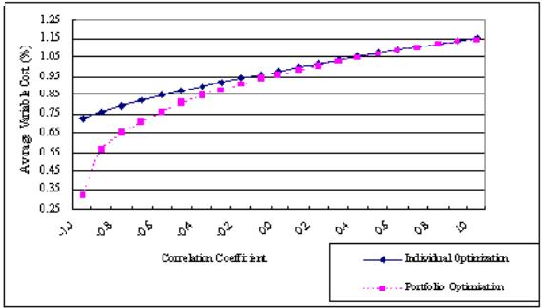
\includegraphics[width=10cm,height=6cm]{fg_b1n.png}
\end{center}
\caption[Correlation coefficient and variable cost in two asset case]{{\bf Correlation coefficient and variable cost in two asset case.}
 \quad This graph shows how variable cost ($y$-axis) changes according to the correlation coefficient
($x$-axis), using market impact coefficients and volatility of typical two stocks.
 Due to diversification effect, simultaneous optimization reduces cost than iterative optimization
($V_1=100$, $V_2=150$, $a_1=0.0002$, $a_2=0.0003$, $\sigma_1=0.001$, $\sigma_2=0.0015$,
$\lambda=1$).}\label{fg_b1}
\end{figure}

%%%%%%%%%%%%%%%%%%%%%%%
\section{Limit to Instantaneous Executable Volume}\label{sec_b4}

\noindent 1) Solution with upper limit 

 So far, we have assumed market impact is linear.  However, in practice, this does not always hold without any restrictions, but only within moderate trading volume and time.  Therefore, in this section, we consider the effect of limit to the volume executable instantaneously.  For simplicity, we study only single asset case.  Without limit, recall that the optimal execution strategy as well as average variable cost have been obtained in Proposition \ref{cor_b1}.

 Now, assume that there is an upper limit $V_0$ to the volume executable instantaneously.  The solution in the above violates the limit when
\begin{equation}\label{eq_b20}
  v(0)=\left( \frac{\lambda^2 \sigma^2 V}{2a^2} \right)^{1/3} > V_0, \qquad
  \mbox{or\ equivalently,} \qquad V>\frac{2a^2V_0^3}{\lambda^2\sigma^2}.
\end{equation}
 If this is the case, it seems difficult to get an explicit form of the optimal solution.  However, since the price movement risk is an increasing function of time while market impact coefficient remains constant, $v(t)$ is considered to be a decreasing function of time.  Therefore, the optimal execution strategy is expected to take a constant value $V_0$ on $[0,t_0]$ and then decrease monotonically to approach zero asymptotically.  Thus, it is natural to approximate the optimal execution strategy as
\begin{equation}\label{eq_b18}
  v_0(t) = \left\{
  \begin{array}{ll}
   V_0, & \quad 0 \leq t < t_0, \\
   V_0 e^{-\beta (t-t_0)}, & \quad t_0 \leq t.
  \end{array}
  \right.
\end{equation}
 From the constraint (\ref{eq_b1}),
\[
  V = \int_0^\infty v_0(t) dt = V_0 \left( t_0 + \frac{1}{\beta} \right)
\]
so that the relation
\begin{equation}\label{eq_b19}
  \beta = \frac{V_0}{V-V_0t_0}
\end{equation}
holds.
 The following proposition identifies optimal $t_0$ (and hence $\beta$) for this approximation.

\begin{proposition}\label{prop_b2}
 \quad Within function class that satisfies (\ref{eq_b18}) and (\ref{eq_b19}),
the optimal $t_0$ is given as a unique solution of
\begin{equation}\label{eq_b30}
  \left(t_0-\gamma\right)^4 + \frac{2a^2V_0^2}{3\lambda^2\sigma^2}
  \left\{ \left( t_0 - \gamma \right)^3-2 \gamma^3 \right\} = 0, \quad
  t_0 \in (0, \gamma);
  \qquad \gamma=\frac{V}{V_0}.
\end{equation}
\end{proposition}
\begin{proof}
  See Section \ref{sec_bappendix}.
\end{proof}

\noindent In order to see the precision of the approximation, we compare the numerical solution and this approximation with real market data.  Figure \ref{fg_b2} shows the optimal execution strategy of stock 1 in the Section \ref{sec_b3}.  The limit to instantaneous execution volume is assumed to be 10 units since the average trading volume was 32 units in that period, and we regard market share over 30\% is too much ($\sigma=0.001$, $a=0.0002$, $\lambda=1$, $V=200$, $V_0=10$).  Figure \ref{fg_b2} supports this approximation.

\begin{figure}[htbp]
\begin{center}
 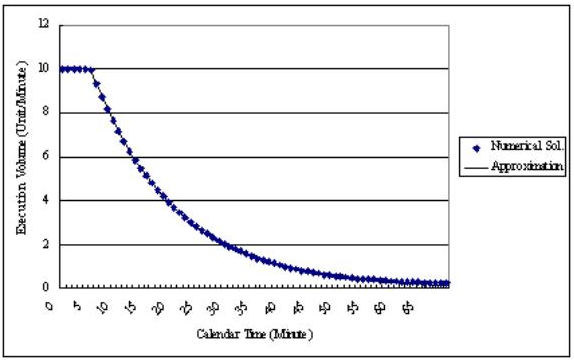
\includegraphics[width=10cm,height=6cm]{fg_b2n.png}
\end{center}
\caption[Numerical solution and approximation for the case with upper limit]{{\bf Numerical solution and approximation for the case with upper limit.}
 \quad Instantaneous execution volume of numerical solution (dashed curve) and approximation (solid curve)
of the optimal execution strategy of the stock in the Section \ref{sec_b3} is on $y$-axis, and time is on $x$-axis.
 The limit to instantaneous execution volume is assumed to be 10.  Approximation is good enough to be
almost indistinguishable with numerical solution.  ($\sigma=0.001$, $a=0.0002$, $\lambda=1$, $V=200$,
$v_0=10$).}\label{fg_b2}
\end{figure}

 For multiple asset case, we can expect an exponential function as we did in the one asset case.  However, the formula of opportunity cost depends on the integration range, and so we need to calculate case by case according to the time when the execution volume of each asset becomes variable.

\bigskip

\noindent 2) Numerical examples

 It is difficult to identify implications on sensitivity of parameters and constraints from the optimal strategies since they require numerical calculation.  So, we study the characteristics of the optimal execution strategy of a single asset case.  Specifically, using parameters of stock 1 in Section \ref{sec_b3}, we observe how average variable cost changes according to whole trading size, and compare each solution.  In this comparison, we also show the behavior of optimal execution strategy in which orders are executed at a constant rate (constant execution henceforth) presented in the following proposition.

\begin{proposition}\label{prop_b3}
 \quad Within constant executions, the optimal execution volume $v_c$ is
\[
  v_c = \left\{
  \begin{array}{ll}
   \left( \frac{\lambda^2 \sigma^2 V}{12a^2} \right)^{1/3},
     & \quad V \leq \frac{12 a^2 V_0^3}{\lambda^2 \sigma^2}, \\
   V_0, & \quad V > \frac{12 a^2 V_0^3}{\lambda^2 \sigma^2}
  \end{array}
  \right.
\]
where, as before, $V_0$ is the upper limit to the volume executable instantaneously.
 In this case, the average variable cost is
\[
  \frac{VC}{V} = \left\{
  \begin{array}{ll}
   \left( \frac{9}{4} a \lambda^2 \sigma^2 V \right)^{1/3},
    & \quad V \leq \frac{12a^2V_0^3}{\lambda^2\sigma^2}, \\
   \left( \frac{\lambda^2\sigma^2V}{3V_0} \right)^{1/2}+aV_0,
    & \quad V > \frac{12a^2V_0^3}{\lambda^2\sigma^2}.
  \end{array}
  \right.
\]
\end{proposition}

\begin{proof}
  See Section \ref{sec_bappendix}.
\end{proof}

\noindent Comparing with Proposition \ref{cor_b1}, the average variable cost under constant execution looks quite similar to that of the general optimal execution strategy (general execution henceforth) for small trading size, but the size is
$(4/3)^{1/3}$ times larger.  Figure \ref{fg_b3} and Figure \ref{fg_b4} show the relationship with whole trading size and average variable cost, using parameters of stock 1 in Section \ref{sec_b3} ($\sigma=0.001$, $a=0.0002$, $\lambda=1$, $V_0=10$).

\begin{figure}[htbp]
\begin{center}
 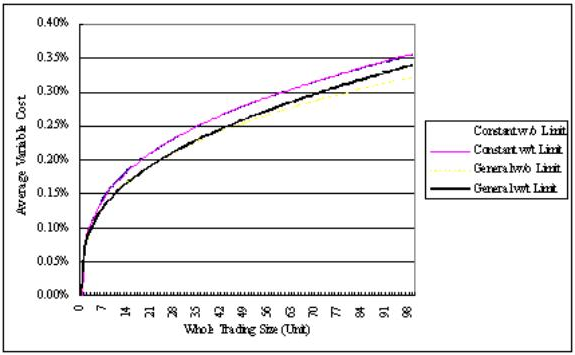
\includegraphics[width=10cm,height=6cm]{fg_b3n.png}
\end{center}
\caption[Whole trading size and average variable cost (small trades)]{{\bf Whole trading size and average variable
cost (small trades).}
 \quad Average variable cost ($y$-axis) is an increasing function of whole trading size ($x$-axis), while the marginal
increment is a decreasing function, which are consistent with intuition.
 Constant execution with limit coincides with constant execution without limit for small trades.
 The same parameters of the stock in Section \ref{sec_b3} are used ($\sigma=0.001$, $a=0.0002$, $\lambda=1$, $V_0=10$).}\label{fg_b3}
\end{figure}

\noindent In Figure \ref{fg_b3}, as long as optimal execution volume is below the limit, average variable costs with and without limit coincide and increase as whole trading size to the power of $1/3$.

\begin{figure}[htbp]
\begin{center}
 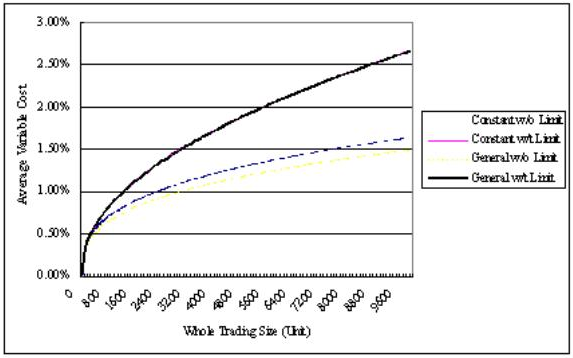
\includegraphics[width=10cm,height=6cm]{fg_b4n.png}
\end{center}
\caption[Whole trading size and average variable cost (large trades)]{{\bf Whole trading size and average variable
cost (large trades).}
 \quad Same graph as Figure \ref{fg_b3}, but for large trades.
 As whole trading size grows, general execution with limit departs from general execution without limit and
approaches constant execution with limit.}\label{fg_b4}
\end{figure}

\noindent As whole trading size grows in Figure \ref{fg_b4}, average variable cost of general execution with limit departs from that of general execution without limit and approaches that of constant execution with limit, which increases as whole trading size to the power of $1/2$.

Further, it is of great interest to compare our optimal execution strategy with those in previous studies such as Almgren and Chriss (1999).  To do so, using parameters on Section 4.4 in Almgren and Chriss (1999), we calculate optimal strategies of both ours and theirs.  They assumed whole trading size $V$ as $10^6$ shares, daily volatility $\sigma$ as $0.95(\$/\mbox{share})/\mbox{day}^{1/2}$, temporary market impact coefficient $a$ as $2.5 \times 10^{-6}(\$/\mbox{share})(\mbox{share}/\mbox{day})$, and risk premium $\lambda$ as $1.645$ for VaR-model and $10^{-6}/\$$ for Variance-model.  Also, the number of time periods was set to five.  We neglect other parameters for simplicity.  Optimal execution strategies are shown in Figure \ref{fg_b5}.  

\begin{figure}[htbp]
\begin{center}
 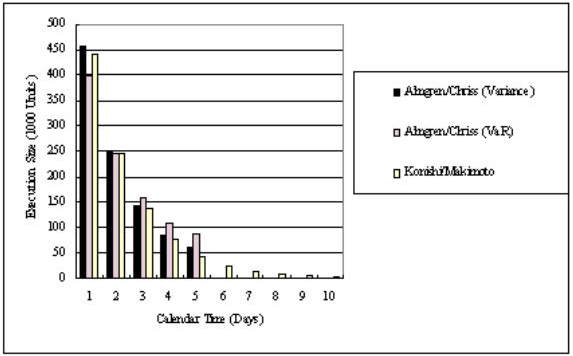
\includegraphics[width=10cm,height=6cm]{fg_b5n.png}
\end{center}
\caption[Comparison of optimal execution strategy.]{{\bf Comparison of optimal execution strategy.}
 \quad Daily execution volume is on $y$-axis, and calendar time is on $x$-axis.
 We can see that, in strategy of Almgren and Chriss (1999), trades which would have best fitted periods after 6 are
somewhat awkwardly pushed into period 3--5 since the number of time
 periods is arbitrarily set to five ($V=10^6$ shares, $\sigma=0.95\mbox{(dollar/share)/day}^{1/2}$, $a=2.5 \times 10^{-6} \mbox{(dollar/share)/day}^{1/2}$, $\lambda =1.645$).}\label{fg_b5}
\end{figure}

\noindent We can see that, in optimal execution strategy of Almgren and Chriss (1999), trades which would have best fitted periods after 6 are somewhat awkwardly pushed into period 3 -- 5 since the number of time periods is arbitrarily set to five.  Further, average variable cost is \$2.18 for our strategy and \$2.60 for that of Almgren and Chriss (1999), and therefore, we can confirm that our model indeed provides lower average cost.

In practice, we suffer statistical errors in estimating parameters.  However, empirical studies such as Uno and Yamada (1993) reports that the market impact coefficients and the price volatilities are rather stable.  Also, it is more realistic to regard parameters stochastic.  However, according to the analysis by Hisata and Yamai (2000) on constant execution, this change does not affect the result significantly.


%%%%%%%%%%%%%%%%%%%%%%%%%
\section{Principle of Optimality}\label{sec_b5}

 In general, optimal policy satisfies the ``principle of optimality," which means that the remaining decision must be the same as the decision taken at the beginning.  However, if we recalculate the optimal execution strategy in Proposition \ref{prop_b1} at halfway, the result differs from the strategy calculated at the beginning.  This is because VaR is not additive regarding time, or standard deviation of price movement is not additive.  This problem might be resolved by introducing a new risk measure although it is often difficult to provide such measure with an exact economical meaning.  For example, standard deviation type measure which ignores historical profit and loss can be defined as
\[
  VC = a \int_0^\infty x'(t)^2 dt + \lambda \sigma \int_0^\infty x(t) dt.
\]
 Here, by Euler's Equation of the calculus of variations,
\[
  -2ax''(t) + \lambda \sigma = 0.
\]
 So, with the initial condition $x(0)=V$,
\[
  v(t) = -x'(t) = \left\{
  \begin{array}{ll}
   - \frac{\lambda \sigma}{2a}t + \sqrt{\frac{\lambda \sigma V}{a}},
     & \quad 0 \leq t < \sqrt{\frac{4aV}{\lambda\sigma}}, \\
   0, & \quad \sqrt{\frac{4aV}{\lambda\sigma}} \leq t.
  \end{array}
  \right.
\]
 We can see that this function satisfies the principle of optimality.
 The average variable cost is,
\[
  \frac{VC}{V} = \frac{4}{3} \sqrt{a \lambda \sigma V}.
\]
 Further, if there is a limit $V_0$ to instantaneous execution volume,
\[
  v(t) = \left\{
  \begin{array}{ll}
   V_0, & \quad 0 \leq t < \frac{V}{V_0}-\frac{aV_0}{\lambda \sigma}, \\
   -\frac{\lambda\sigma}{2a}t + \frac{\lambda\sigma V}{2aV_0} + \frac{V_0}{2},
       & \quad \frac{V}{V_0}-\frac{aV_0}{\lambda \sigma} \leq t < \frac{V}{V_0}+
         \frac{aV_0}{\lambda \sigma}, \\
   0, & \quad  \frac{V}{V_0}+\frac{aV_0}{\lambda \sigma} \leq t
  \end{array}
  \right.
\]
and
\[
  \frac{VC}{V} = \frac{\lambda\sigma V}{2V_0} + aV_0 - \frac{a^2V_0^3}{6\lambda\sigma V}.
\]
 This value increases almost linearly as $V$ increases, which still contradicts the empirical results
of BARRA (1997) and Mannen and Uno (2000).

%%%%%%%%%%%%%%%%%%%%
\section{Closing Remarks}\label{sec_b6}

This chapter has studied execution scheduling of liquidation of a block trade and formulated it as a static optimization problem.  Based on empirical studies on market microstructure, we have distinguished between temporary market impact and permanent market impact, and assumed that each component to be a linear function of trading volume within moderate volume and time.  Also, we have defined the measure of opportunity cost as standard deviation of price movement, and minimized transaction cost, sum of execution cost and opportunity cost.  Under this framework, we have obtained explicit solutions both for the single-asset case and a multiple-asset portfolio model in the form of pure exponentials.  Further, we have derived an approximation formula when there is a limit to the trading volume
executable instantaneously.  

As a result, we have shown that the optimal execution strategy is independent of permanent impact, that optimal execution duration is an increasing function of whole trading size, and that the optimal average cost is an increasing function of whole trading size, price volatility, and temporary impact, and a decreasing function of the limit to instantaneous execution volume, which are all consistent with trading practice and empirical studies.  Specifically, optimal average cost increases as whole trading size to the power of $1/3$ for small orders and $1/2$ for large orders.  Further, it is shown that the transaction cost can be lowered by making order execution late when price movement risk of a portfolio is well diversified.

Our results are immediately applicable to existing risk management framework and provides explicit solution for minimum L-VaR.  Also, although this chapter uses an example of liquidation of a block of common stock, results can be extended over wider problems on liquidation of any large block of assets.

 While this chapter has focused on static optimization, decision change in accordance with new information might be handled by dynamic programming.  Also, this model can reflect more reality by making volatility and market impact time dependent.  Further, it is an interesting issue how to relate order slicing strategy and choice between market order and limit order, and how to control information effect of orders.  These issues are left for further analysis.

\bigskip
\bigskip




%%%%%%%%%%%%%%%%%%%%%%%%
\section{Appendix}\label{sec_bappendix}
\subsection{Proof of Lemma \ref{lem_b3}}
Since $\S$ is non-negative definite, $E \geq 0$ is clear.  Thus, it is enough to prove $EG \geq F^2$.  Non-negative definiteness of $\S$ also implies each eigenvalue $\xi_i\ (i=1,\cdots,N)$ of $\S$ is non-negative (c.f., Bellman (1997), Ch.4.8, Theorem 3).
 This and symmetricity of $\S$ ensure the existence of an orthogonal matrix $\H$ for which
$\S = \H \mbox{Diag}(\xi_1,\cdots,\xi_N) \H^\top$ holds.
 Therefore, if we define $\Q = \H \sqrt{\J} \H^\top$ with $\sqrt{\J} = \mbox{Diag}(\sqrt{\xi_1},\cdots,
\sqrt{\xi_N})$, then $\Q$ is symmetric and $\Q^2=\S$.
 Let $\u(t) = \Q \x(t)$ and $\w(t) = \Q \y(t)$.
 Then, we get
\[
  \x(t)^\top \S \x(t) = \u(t)^\top \u(t), \qquad
  \y(t)^\top \S \y(t) = \w(t)^\top \w(t), \qquad
  \x(t)^\top \S \y(t) = \u(t)^\top \w(t).
\]
 By Cauchy-Schwartz's inequality (cf., Kolmogorov and Fomin (1970)),
%\begin{equation}\label{eq_b11}
%  \x(t)^\top \S \x(t) \cdot \y(t)^\top \S \y(t) \geq [ \x(t)^\top \S \y(t) ]^2.
%\end{equation}
% Since both $\x(t)^\top \S \x(t)$ and $\y(t)^\top \S \y(t)$ are non-negative,
%(\ref{eq_b11}) implies
%\[ %begin{equation}\label{eq_b12}
%  \sqrt{\x(t)^\top \S \x(t)} \cdot \sqrt{\y(t)^\top \S \y(t)} \geq
%  | \x(t)^\top \S \y(t) |
%\] %\end{equation}
%which together with Schwartz's integral inequality show
\begin{eqnarray*}
  \left( \int_0^\infty \x(t)^\top \S \x(t) dt \right)
  \left( \int_0^\infty \y(t)^\top \S \y(t) dt \right)
  & = & 
   \left( \int_0^\infty \u(t)^\top \u(t) dt \right)
   \left( \int_0^\infty \w(t)^\top \w(t) dt \right) \\
  & \geq & \left( \int_0^\infty \u(t)^\top \w(t) dt \right)^2 \\
  & = & \left( \int_0^\infty \x(t)^\top \S \y(t) dt \right)^2,
\end{eqnarray*}
completing the proof.


\subsection{Proof of Proposition \ref{prop_b2}}
 For notational simplicity, we calculate $VC/V_0^2$ instead of $VC$.
 Let $\gamma = V/V_0$.
 Then, from (\ref{eq_b18}) and (\ref{eq_b19}),
\[
  \int_0^\infty \frac{v_0(t)^2}{V_0^2} dt = 
  \left[ \int_0^{t_0} dt + \int_{t_0}^\infty e^{-2\beta(t-t_0)} dt \right]
  = \frac{t_0+\gamma}{2}.
\]
 Further, if we let $x_0(t) = \int_t^\infty v_0(s) ds$,
\[
  \frac{x_0(t)}{V_0}
   = \left\{
   \begin{array}{ll}
    \gamma - t, & \quad 0 \leq t < t_0, \\
    \beta^{-1} e^{-\beta(t-t_0)}, & \quad t_0 \leq t.
   \end{array}
   \right.
\]
 So,
\[
  \int_0^\infty \frac{x_0(t)^2}{V_0^2} dt
   = \int_0^{t_0} (t-\gamma)^2 dt + \int_{t_0}^\infty \beta^{-2}
     e^{-2\beta (t-t_0)} dt
   = -\frac{1}{6} (t_0 - \gamma)^3 + \frac{1}{3} \gamma^3.
\]
 Therefore,
\begin{equation}\label{eq_b31}
  \frac{VC}{V_0^2} = \frac{a(t_0+\gamma)}{2} + \frac{\lambda \sigma}{\sqrt{6}\,V_0}
  \sqrt{-(t_0-\gamma)^3+2\gamma^3} =: f(t_0).
\end{equation}
 Note that the range of $f(t_0)$ is $t_0 \in (0,\gamma)$ from (\ref{eq_b18}).
 Since the first term of $f(t_0)$ linearly increases as $t_0$ increases while the second
term is a convex decreasing function, $f(t_0)$ is convex.
 Moreover,
\[
  f'(t_0) = \frac{1}{4} \left\{ 2a - \frac{\lambda \sigma}{\sqrt{6} \, V_0}
  \frac{(t_0-\gamma)^2}{\sqrt{-(t_0-\gamma)^3+2\gamma^3}} \right\}.
\]
 Then,
\begin{eqnarray*}
  & & f'(0) = \frac{1}{4} \left( 2a - \frac{\sqrt{2\gamma}\lambda\sigma}{V_0} \right) < 0, \qquad
              \mbox{(from (\ref{eq_b20}))} \\
  & & f'(\gamma) = \frac{a}{2} > 0.
\end{eqnarray*}
 Summarizing these arguments, we conclude that $t_0$ that minimizes $VC/V_0^2$ is given
as a unique solution of $f'(t_0)=0$, $t_0 \in (0,\gamma)$.
 Rearranging terms, the desired result is obtained.

%%%%%%%%%%%%%%%
\subsection{Proof of Proposition \ref{prop_b3}}
 Consider a constant execution in which orders are executed at a constant volume $v_c$ until time $t_0$.
 According to the constraint in (\ref{eq_b1}), $v_c$ and $t_0$ satisfy
\begin{equation}\label{eq_b32}
  \int_0^{t_0} v_c dt = v_c t_0 = V, \qquad \mbox{or} \qquad v_c = \frac{V}{t_0}.
\end{equation}
 Noting that
\[
  x(t) = \left\{
  \begin{array}{ll}
   (t_0-t)v_c, & \quad 0\leq t\leq t_0, \\
   0, & \quad t_0 < t,
  \end{array}
  \right.
\]
the total cost can be calculated as
\[
  VC = a \frac{V^2}{t_0} + \lambda \sigma V \sqrt{\frac{t_0}{3}}.
\]
 Therefore, the optimal $t_0$ that minimized the variable cost is
\[
  t_0 = \left( \frac{12a^2V^2}{\lambda^2\sigma^2} \right)^{1/3},
\]
and, from (\ref{eq_b32}), the optimal execution volume is
\[
  v_c = \left( \frac{\lambda^2 \sigma^2 V}{12a^2} \right)^{1/3}.
\]
 Also, average variable cost becomes
\[
  \frac{VC}{V} = \left( \frac{9}{4} \lambda^2 \sigma^2 aV \right)^{1/3}.
\]
 When there is a limit $V_0$ to instantaneous execution volume, $t_0$ needs to satisfy
$t_0 \geq V/V_0$.
 In summary, the optimal execution period is given as
\[
  t_0 = \max \left( \left( \frac{12a^2V^2}{\lambda^2\sigma^2} \right)^{1/3}, \frac{V}{V_0} \right)
\]
and the desired results can be obtained by a straightforward calculation.
